\chapter{Addendum}
\label{Addendum}

\section{Issues Encountered}
At the time this report was submitted, the augmented reality subsystem was incapable of showing positions. A full analysis of the project's systems was conducted. The following issues were discovered and corrected:

\begin{enumerate}
	\item The rangefinding subsystem was found to have a subtle timing bug which would cause the data being sent to overwrite the received data in the DWM1000's data buffer. The device would then believe it had received a message from a new device, and add its own ID twice to the transmission order array. It would then interfere with the network by taking its turn twice.
	
	To fix this, a method was discovered to optimize parsing of data and give the device more time to work with before it would be expected to transmit. 
	
	The Arduino's \code{Serial.print} function was called multiple times to output the ranges to the cell phone, but this function has a very high fixed cost independent of the length of data transmitted. It was found that outputted ranges being concatenated in a String before making a single call to \code{Serial.println} improved performance almost twice over for some numbers of devices. This extra time solved the timing bug. 
	\item The position calculation subsystem had several issues:
	\begin{enumerate}
		\item Due to floating point math errors, it was quite common for any formulas using $\arccos$ to be given values greater than 1 or less than -1. This would result in NaN positions. A function to clamp values within this range fixed this bug.
		\item There was a rare case where rotating the temporary point of anchor 4 around the x axis would result in the equation being unsolvable. Checks were added to ensure that the value passed to $\arccos$ were within the range of $[-1, 1]$.
		\item In order to calculate z-values appropriately, the four anchors cannot be co-planar. It was discovered that the four anchors were mistakenly placed very nearly coplanar during testing. This triggered the rotation bug much more than it otherwise had before.
	\end{enumerate}
\end{enumerate}

With the above issues fixed, the system was able to work once more.

\section{Augmented Reality Results}
\begin{figure}
	\centering
	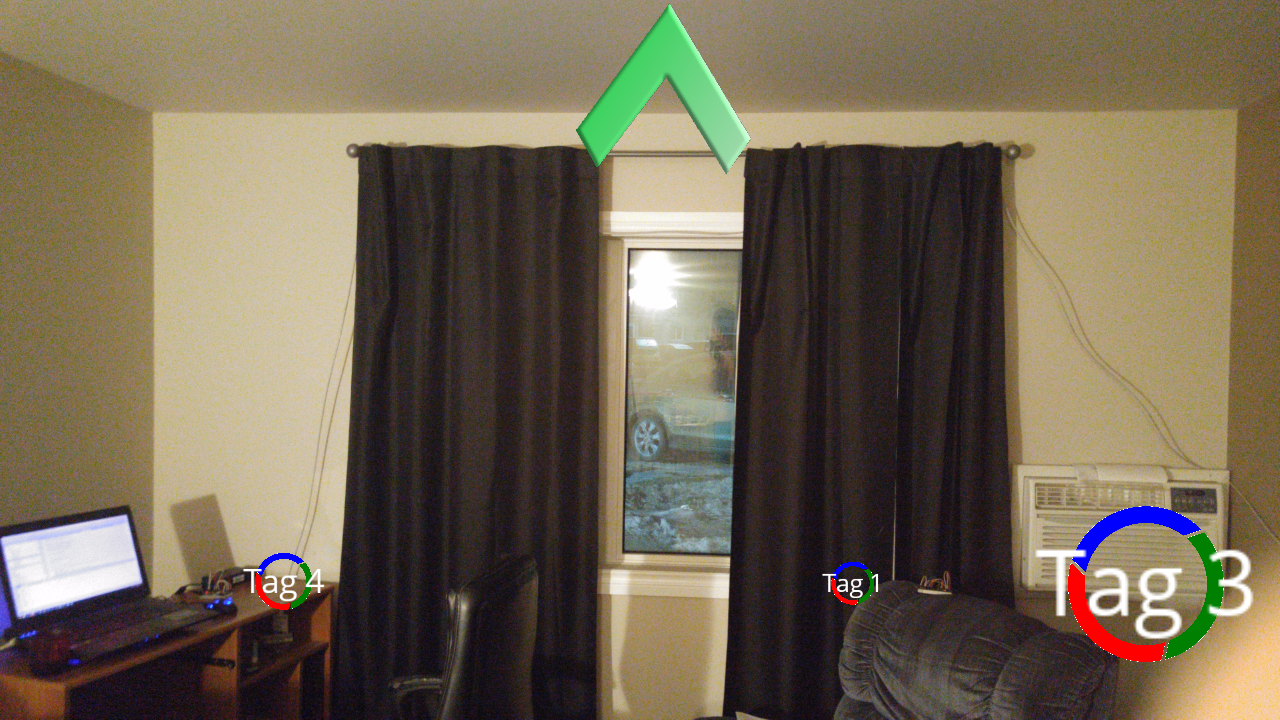
\includegraphics[width=\linewidth]{Figures/AR1.png}
	\decoRule
	\caption{After being calibrated, the system displays the position of two tags relatively accurately and a third inaccurately. Note the HUD arrow at the top of the screen pointing to an anchor directly behind the cell phone.}
	\label{fig:AR1}
\end{figure}

Figure~\ref{fig:AR1} shows an example of the system in use. An anchor is on the computer desk, just above the mouse, and on the chair to the right. As can be seen, the system is incorrectly displaying the position of Tag 3 - it should not be on the screen. It is, however, within 3m of the actual position.

It was discovered that positions are generally within a meter or two of the object in question, however this varies greatly. The displayed positions were subject to great noise.

The system freezes for 200ms or more every time positions are calculated, giving a little less than 5Hz position update frequencies and at least a 200ms update latency. This is due to positions not being calculated in their own thread. Time constraints did not allow this optimization in time for the writing of this addendum. Still, this update frequency is above the minimum requirement of a 1Hz update frequency.

\section{Overall Performance Metrics}

Table~\ref{tab:OverallResults} lists the project's performance metrics compared to the requirements.

\begin{table}
\caption{System performance metrics vs. required minimum metrics}
\label{tab:OverallResults}
\centering
\begin{tabular}{c c c}
\toprule
\tabhead{Metric} & \tabhead{Minimum Required} & \tabhead{Measured} \\
\midrule
Sensor Accuracy & Within 3m & Within 1-2m \\
Sensor Range & At least 5m & Over 10m, theorized 60m \\
Battery Life & At least 15 minutes & 1-2 hours \\
Location Update Frequency & 1Hz & 5Hz \\
Location Update Latency & Under 1000ms & $\approx$200 ms \\
\bottomrule 
\end{tabular}
\end{table}

\section{Corrections}
\begin{figure}
	\centering
	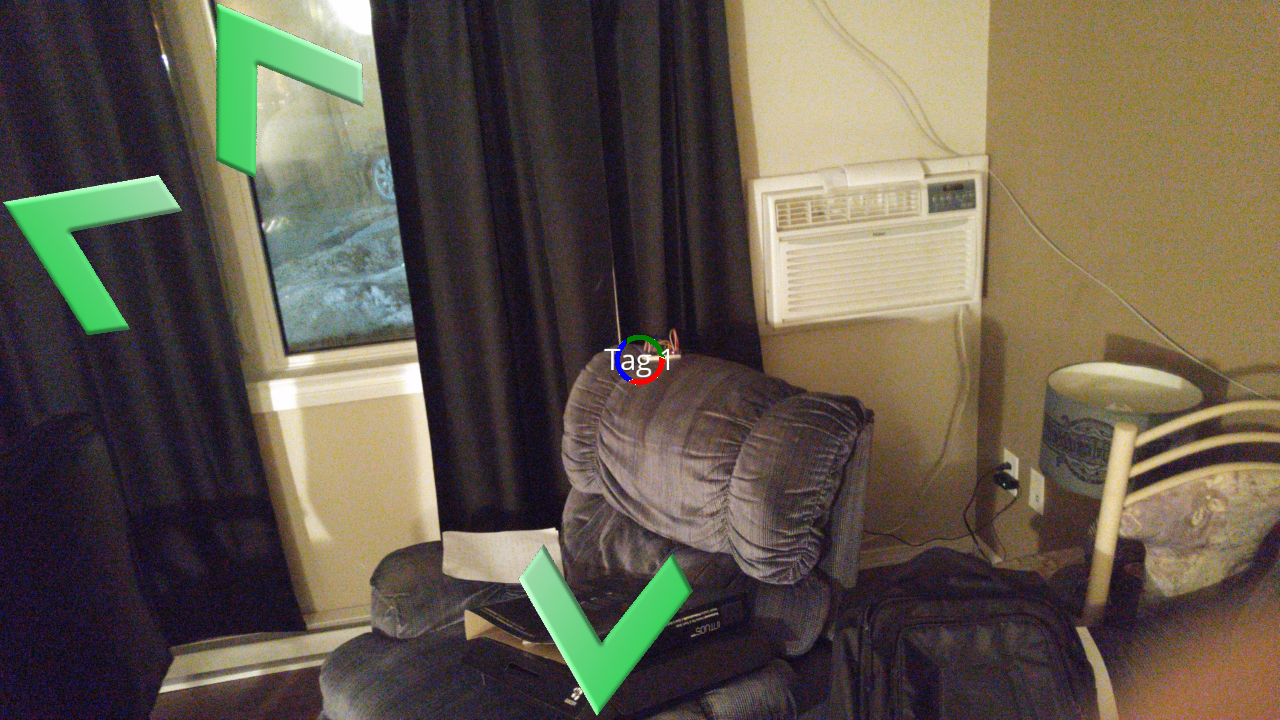
\includegraphics[width=\linewidth]{Figures/CalFinal.png}
	\decoRule
	\caption{An image showing the calibration process. Tag 1 is centered on the screen, and the user must align it with the actual tag 1.}
	\label{fig:CalFinal}
\end{figure}
Due to the system failure delaying editing, this report contains a number of errors. A brief listing of them is presented below.

\begin{enumerate}
	\item The abstract is incorrect; positions displayed via the AR display are much more inaccurate than the rangefinding subsystem's values. This is due to a combination of slightly incorrect rendering and errors accumulated during position calculations.
	\item The calibration images in Figures~\ref{fig:Cal1} and \ref{fig:Cal2} are using dummy values, not actual values obtained from the position calculation subsystem. An updated image showing calibration of Tag 1 can be seen in Figure~\ref{fig:CalFinal}.
	\item In Chapter~\ref{AugmentedReality} it should be stated that the model matrix for each tag is simply a translation matrix of the tag's position minus the position of the tag connected to the cellphone. A billboarding effect is also applied to the model matrix.
	\item Though implicitly, it should be explicitly noted that the model, view, and projection matrix are applied in order. That is, for every vertex $v$ to be drawn for the objects in the scene, it is transformed into $v'$ with the equation
	
	\[ v' = \mathbf{P}\mathbf{V}\mathbf{M}v \]
\end{enumerate}
